% Short note on the spray-exposure score S (revision 5). Build: `make here` -> build/scoring_note.pdf
\documentclass[10pt]{article}
\usepackage[a4paper,hmargin=1.7cm,vmargin=1.2cm]{geometry}
\usepackage{amsmath,amssymb,booktabs,enumitem}
\usepackage{graphicx}
\usepackage{tikz}
\usetikzlibrary{arrows.meta,decorations.pathreplacing}
\setlist{itemsep=1pt,topsep=2pt,parsep=0pt}
\setlength{\parindent}{0pt}
\setlength{\parskip}{4pt}
\setlength{\emergencystretch}{1em}
\pagestyle{empty}

% notation (the figures use \vp, \vn, \vq)
\newcommand{\vect}[1]{\mathbf{#1}}
\newcommand{\vp}{\vect{p}}
\newcommand{\vn}{\vect{n}}
\newcommand{\vq}{\vect{q}}
\newcommand{\vs}{\vect{s}}
\newcommand{\vd}{\vect{d}}
\newcommand{\vm}{\vect{m}}
\newcommand{\Occ}{\mathcal{G}}
\newcommand{\ind}{\mathbb{I}}
\newcommand{\head}[1]{\par\smallskip\textbf{#1}\quad}
% Hidden detail: how the K spray points are spread on a disc. Kept in the source, not printed.
% Change \discdetailfalse to \discdetailtrue to print it (Step 2 and the extra Fig. 2 disc panel).
\newif\ifdiscdetail
\discdetailfalse
% Hidden: the puddle rule (Section 1 sentence, Section 2 block, delta_p) and the properties list.
% Change ...false to ...true to print them.
\newif\ifpuddlerule
\puddlerulefalse
\newif\ifproperties
\propertiesfalse
% a figure inside a step of Section 2: centered at its natural size, caption below
\newcommand{\mathfig}[3]{\par\smallskip{\centering #2\\[2pt]
  \parbox{0.92\linewidth}{\footnotesize\textbf{Fig.~#1.} #3}\par}\medskip}

\begin{document}
\setlength{\abovedisplayskip}{4pt}\setlength{\belowdisplayskip}{4pt}
\setlength{\abovedisplayshortskip}{2pt}\setlength{\belowdisplayshortskip}{2pt}

{\LARGE\bfseries How a dishwasher load is scored ($S$)}\\[3pt]
{\small Spray-exposure score, revision~5 \,\textperiodcentered\, HOTEC $\times$ Frigidaire benchmark \,\textperiodcentered\, 2026-09-27}

\medskip
\textbf{In one sentence:} $S$ is the average, over all food-contact surface in the racks (each dish weighted by its area), of how much of the part of its spray-arm disc in front of it the surface sees in a straight line, head-on directions counting more.
It runs from $0$ to $1$; higher is better.

\section*{1\quad The idea}
\begin{enumerate}
\item \textbf{Dots.} Put 500 dots on each dish's food-contact surface (the inside of a bowl or cup, the top of a plate), spread in proportion to area.
\item \textbf{Lines.} From each dot, draw a straight line to each of the 64 spray points on the disc that the spray arm under its rack sweeps.
\item \textbf{Dot score $e$.} Ignore lines that come from behind the surface. Of the rest, $e$ is the share that reach their spray point without hitting anything (another dish, the dish itself, a rack or basket wire). Head-on lines count more than grazing ones; if no line is in front, $e=0$.
\item \textbf{Dish score $E$.} Average $e$ over the dish's 500 dots.
\item \textbf{Load score $S$.} Average $E$ over the racked dishes, weighting each dish by its food-contact area (plate 502, bowl 340, cup 215\,cm$^2$).
\end{enumerate}
\ifpuddlerule
A load in which any plate, bowl or cup would hold a puddle is \emph{infeasible}, whatever its $S$.
\fi

\small
\setlength{\abovedisplayskip}{3pt}\setlength{\belowdisplayskip}{3pt}
\section*{2\quad The math}
Each block below gives the math of the step with the same number in Section~1, and one figure that draws its symbols. Figs.~1, 4 and 5 use a real load (the hard-tier goal load of the benchmark, 23 dishes); Fig.~2 is a schematic, and Fig.~3 uses the real lower-arm disc with a hand-made example.

\head{Step 1: Dots.}
We score one loading of the dishwasher, called an arrangement $X$; only dishes inside a rack count, and $\mathcal{O}_X$ is that set, with $o$ one dish.
Each dish is represented by $N$ dots spread in proportion to area over its food-contact surface (the inside of a bowl or cup, the top of a plate).
Dot $j$ has a position $\vp_j$ and a unit normal $\vn_j$ pointing away from the dish material (into the cavity of a bowl or cup, out of a plate's eating face), both in dishwasher coordinates (see the end of the note), and stands for the area $A_o/N$, where $A_o$ is the food-contact area of its dish (plate 502, bowl 340, cup 215\,cm$^2$).
One index $j$ numbers the dots of all racked dishes together, and $\mathcal{J}_o$ is the set of indices of dish $o$'s dots.
Bold letters are vectors, and $\vect a^\top\vect b$ is the dot product of $\vect a$ and $\vect b$.
A spray line is blocked if it hits $\Occ(X)$: a wire of either rack or of the cutlery basket, or any racked dish, including the dish being scored (the tub walls and door never block).

\mathfig{1}{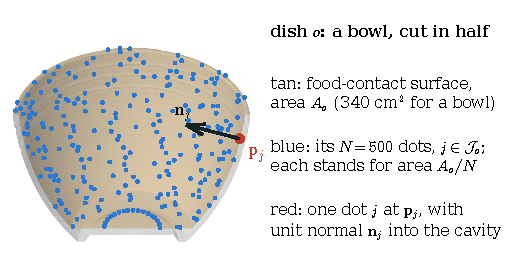
\includegraphics{figures/step1_dots.pdf}}
{Step 1 in symbols, on a real bowl (cut in half, drawn upright). Tan: its food-contact surface, of area $A_o$. Blue: its $N=500$ dots $j\in\mathcal{J}_o$, each standing for the area $A_o/N$. Red: one dot at $\vp_j$ with its unit normal $\vn_j$, pointing into the cavity. The middle of the floor is a fan of 96 large mesh triangles whose centers lie on one circle, so the dots there line up on a ring.}

\head{Step 2: Lines.}
Dish $o$ connects to the spray arm under its rack, $a(o)\in\{\mathrm{low},\mathrm{mid}\}$: the lower arm if it sits in the lower rack or the cutlery basket, the middle arm (under the upper rack) if it sits in the upper rack.
Each arm $a$ is modeled by the flat disc $\mathcal{D}_a$ that it sweeps, which carries $K$ spray points $\vq_k$, $k=0,\dots,K-1$, spread evenly over it, each with the same weight $u_k=1/K$ (the arm is always the dish's arm $a(o)$, so it is left out of the index).
\ifdiscdetail
The disc has center $\vm_a$ and radius $\rho_a$, and the points follow a sunflower pattern:
\begin{equation}
\vq_k=\vm_a+\rho_a\sqrt{(k+\tfrac12)/K}\,\bigl(\cos k\phi,\ \sin k\phi,\ 0\bigr),\qquad \phi=\pi(3-\sqrt5)\approx137.5^\circ,
\end{equation}
where $\phi$ is the golden angle.
The square-root factor puts point $k$ in the ring between radii $\rho_a\sqrt{k/K}$ and $\rho_a\sqrt{(k+1)/K}$, and every such ring has area $\pi\rho_a^2/K$; the golden-angle turns spread the points around the center.
So the $K$ points cover the disc evenly, which is why they get equal weights.

\mathfig{2 (disc detail)}{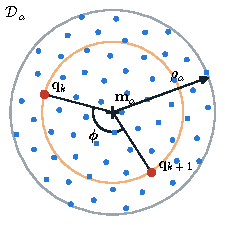
\includegraphics{figures/step2_disc.pdf}}
{Disc $\mathcal{D}_a$ from above, with center $\vm_a$, radius $\rho_a$ and its $K=64$ spray points. The shaded ring $k$ (radii $\rho_a\sqrt{k/K}$ to $\rho_a\sqrt{(k+1)/K}$, area $\pi\rho_a^2/K$) holds exactly one point, $\vq_k$; the next point $\vq_{k+1}$ is turned by the golden angle $\phi$.}
\fi

Now fix a dot $j$ of dish $o$ and a spray point $\vq_k$ of $\mathcal{D}_{a(o)}$; the racks are in their pushed-in (closed) position.
The line starts just off the surface, at $\vs_j=\vp_j+\epsilon\vn_j$ with a small offset $\epsilon$, so that it does not hit its own surface.
Its length is the distance $\ell_{jk}=\lVert\vq_k-\vs_j\rVert$, where $\lVert\cdot\rVert$ is the Euclidean length, and its unit direction is $\vd_{jk}=(\vq_k-\vs_j)/\ell_{jk}$.
The line is \emph{open} when it touches nothing in $\Occ(X)$ before reaching the spray point:
\begin{equation}
v_{jk}=\ind\bigl[\{\vs_j+t\,\vd_{jk}:\ 0<t<\ell_{jk}\}\cap\Occ(X)=\emptyset\bigr].
\end{equation}
Here the set lists the points of the line, $t$ being the distance travelled from $\vs_j$; ``$\cap\,\Occ(X)=\emptyset$'' says that none of them lies on a blocker; and the indicator $\ind[\cdot]$ is $1$ when the statement in brackets is true and $0$ otherwise.
The line's \emph{head-on weight} is the cosine of the angle between the normal and the line, clipped at zero:
\begin{equation}
\gamma_{jk}=\max\bigl(0,\ \vn_j^\top\vd_{jk}\bigr).
\end{equation}
It is $1$ for a line that meets the surface straight on, close to $0$ for a grazing line, and $0$ for a spray point behind the surface (dotted in Fig.~2b).
Spray points with $\gamma_{jk}>0$ are called \emph{front-facing}.

\mathfig{2}{\begin{tabular}{@{}c@{\hspace{8mm}}c@{}}% Fig. 2 (b): one dot and ONE line, with every symbol of Step 2. Hand-computed (cm):
% p = (0, 2.0), n at -20 deg drawn from p (s lies on it); s = p + eps n with eps drawn exaggerated (0.45) -> (0.423, 1.846);
% the line to q_k = (0.6, 0) points at -84.5 deg, so theta = 64.5 deg; tangent plane at 70 deg through p.
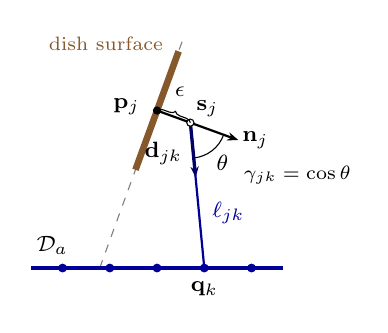
\begin{tikzpicture}[x=1cm,y=1cm,>={Stealth[length=4pt]},font=\footnotesize]
  % tangent plane and the dish surface around the dot
  \draw[gray,dashed] (-0.728,0) -- (0.342,2.94);
  \draw[line width=2.4pt,brown!70!black] (-0.274,1.248) -- (0.274,2.752);
  \node[anchor=east,text=brown!70!black,font=\scriptsize] at (0.2,2.85) {dish surface};
  % the disc, edge-on
  \draw[line width=1.6pt,blue!60!black] (-1.6,0) -- (1.6,0);
  \foreach \x in {-1.2,-0.6,0.0,0.6,1.2} \fill[blue!60!black] (\x,0) circle (1.6pt);
  \node[anchor=south west] at (-1.65,0.05) {$\mathcal{D}_a$};
  \node[anchor=north] at (0.6,-0.05) {$\vq_k$};
  % the line from s_j to q_k: length and unit direction
  \draw[blue!60!black,thick] (0.423,1.846) -- (0.6,0);
  \node[blue!60!black,anchor=west] at (0.58,0.7) {$\ell_{jk}$};
  \draw[->,very thick,blue!40!black] (0.423,1.846) -- (0.490,1.149);
  \node[anchor=east] at (0.44,1.45) {$\vd_{jk}$};
  % angle between the normal and the line
  \draw (0.423,1.846) ++(-20:0.45) arc[start angle=-20,end angle=-84.5,radius=0.45];
  \node at (0.83,1.33) {$\theta$};
  \node[anchor=west,font=\scriptsize] at (0.98,1.18) {$\gamma_{jk}=\cos\theta$};
  % dot, lifted start, normal
  \fill (0,2.0) circle (1.5pt);
  \node[anchor=east] at (-0.1,2.05) {$\vp_j$};
  \draw[->,thick] (0,2.0) -- (1.034,1.624) node[anchor=west,inner sep=1pt] {$\vn_j$};
  \fill[white,draw=black] (0.423,1.846) circle (1.3pt);
  \node[anchor=south west,inner sep=1pt] at (0.46,1.88) {$\vs_j$};
  \draw[decorate,decoration={brace,amplitude=2pt}] (0,2.0) -- (0.423,1.846);
  \node[anchor=south,inner sep=1pt] at (0.29,2.13) {$\epsilon$};
\end{tikzpicture}
 & % Fig. 2 (c): one dot and lines to 8 of the K spray points, side view: open, blocked, behind.
% Hand-computed (cm): n_j at -20 deg; lines start at s_j = p_j + eps n_j (eps exaggerated, 0.35);
% tangent plane through p_j meets the disc at x = -0.6, so points at x <= -1.0 are behind;
% the neighboring dish (x = 1.4..1.6, z = 0.6..3.0) blocks the lines to x = 1.9 and 2.6
% at z = 0.759 and 1.205.
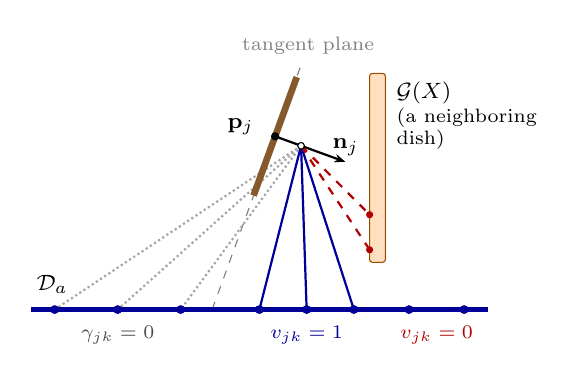
\begin{tikzpicture}[x=1cm,y=1cm,>={Stealth[length=4pt]},font=\footnotesize]
  % tangent plane of the dot
  \draw[gray,dashed] (-0.6,0) -- (0.542,3.14);
  \node[gray,anchor=south,font=\scriptsize] at (0.62,3.12) {tangent plane};
  % blocker: a neighboring dish
  \draw[fill=orange!25,draw=orange!60!black,rounded corners=1pt] (1.4,0.6) rectangle (1.6,3.0);
  \node[anchor=west] at (1.62,2.75) {$\mathcal{G}(X)$};
  \node[anchor=west,font=\scriptsize,align=left] at (1.62,2.3) {(a neighboring\\ dish)};
  % behind the tangent plane: gamma = 0
  \foreach \x in {-2.6,-1.8,-1.0} \draw[gray!70,densely dotted,thick] (0.529,2.080) -- (\x,0);
  % open lines: v = 1
  \foreach \x in {0.0,0.6,1.2} \draw[blue!60!black,thick] (0.529,2.080) -- (\x,0);
  % blocked lines: v = 0, drawn up to the hit
  \draw[red!70!black,thick,dashed] (0.529,2.080) -- (1.4,0.759);
  \draw[red!70!black,thick,dashed] (0.529,2.080) -- (1.4,1.205);
  \fill[red!70!black] (1.4,0.759) circle (1.3pt);
  \fill[red!70!black] (1.4,1.205) circle (1.3pt);
  % disc, edge-on, with its spray points
  \draw[line width=1.6pt,blue!60!black] (-2.9,0) -- (2.9,0);
  \foreach \x in {-2.6,-1.8,-1.0,0.0,0.6,1.2,1.9,2.6} \fill[blue!60!black] (\x,0) circle (1.6pt);
  \node[anchor=south west] at (-2.95,0.08) {$\mathcal{D}_a$};
  \node[gray!60!black,font=\scriptsize] at (-1.8,-0.32) {$\gamma_{jk}=0$};
  \node[blue!60!black,font=\scriptsize] at (0.6,-0.32) {$v_{jk}=1$};
  \node[red!70!black,font=\scriptsize] at (2.25,-0.32) {$v_{jk}=0$};
  % surface patch, dot, normal
  \draw[line width=2.4pt,brown!70!black] (-0.074,1.448) -- (0.474,2.952);
  \fill (0.2,2.2) circle (1.5pt);
  \node[anchor=east] at (0.05,2.32) {$\vp_j$};
  \draw[->,thick] (0.2,2.2) -- (1.093,1.875) node[anchor=south,inner sep=2pt] {$\vn_j$};
  \fill[white,draw=black] (0.529,2.080) circle (1.2pt);
\end{tikzpicture}
\\ {\footnotesize (a) one line} & {\footnotesize (b) all lines of one dot}\end{tabular}}
{Step 2 in symbols, seen from the side with the disc $\mathcal{D}_a$ edge-on.
(a) One dot and one line: the line starts at $\vs_j=\vp_j+\epsilon\vn_j$ ($\epsilon$ drawn far larger than 0.1\,mm), ends at the spray point $\vq_k$, has length $\ell_{jk}$ and unit direction $\vd_{jk}$, and makes the angle $\theta$ with the normal $\vn_j$, so $\gamma_{jk}=\cos\theta$.
(b) All lines of one dot: solid lines are open ($v_{jk}=1$), red dashed lines hit the blocker $\Occ(X)$ ($v_{jk}=0$), and dotted lines go to spray points behind the dot's tangent plane ($\gamma_{jk}=0$).}

\head{Step 3: Dot score.}
With the sums over $k$ running over the $K$ spray points of $\mathcal{D}_{a(o)}$,
\begin{equation}
e_j=\frac{\sum_k u_k\gamma_{jk}v_{jk}}{\sum_k u_k\gamma_{jk}}\qquad\Bigl(e_j=0\ \text{if}\ \textstyle\sum_k u_k\gamma_{jk}=0\Bigr).
\label{eq:e}
\end{equation}
$e_j$ is the \emph{dot exposure}: the head-on-weighted share of its front-facing spray points that the dot sees through open lines.
The equal weights $u_k$ cancel in~\eqref{eq:e}; they are kept for the optional ceiling source mentioned at the end.

\mathfig{3}{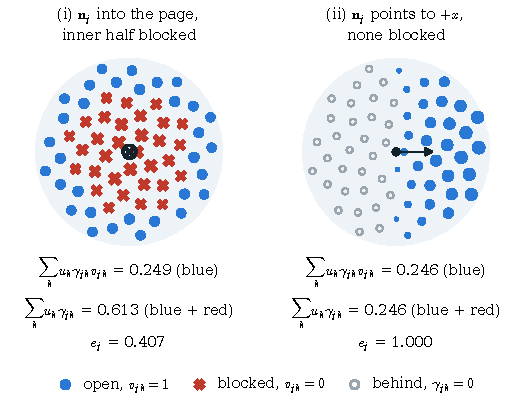
\includegraphics{figures/step3_dot.pdf}}
{Step 3 in symbols, for one dot 115\,mm above the center of the lower disc (top view; blocking set by hand). Point size is proportional to $\gamma_{jk}$.
(i) $\vn_j$ points straight at the disc ($\otimes$) and the 32 most head-on points are blocked: half the points are open, yet $e_j=0.249/0.613=0.407$, because the blocked lines carry the most weight.
(ii) $\vn_j$ points to $+x$ (arrow): the 31 points behind the surface have $\gamma_{jk}=0$ and drop out of both sums, and all 33 in front are open, so $e_j=1$.}

\head{Step 4: Dish score.}
\begin{equation}
E_o=\frac1N\sum_{j\in\mathcal{J}_o}e_j,
\end{equation}
the \emph{dish exposure}: the mean of $e_j$ over the dish's $N$ dots.

\mathfig{4}{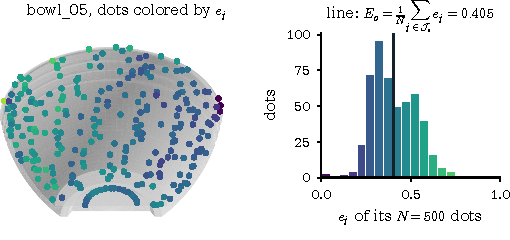
\includegraphics{figures/step4_dish.pdf}}
{Step 4 in symbols, on bowl\_05, the best-sprayed dish of the example load. Left: half of the bowl, drawn upright for readability (in the rack it hangs mouth-down), each dot colored by its $e_j$ in the rack pose. Right: the $e_j$ of all $N=500$ dots $j\in\mathcal{J}_o$; their mean is the dish score $E_o=0.405$.}

\head{Step 5: Load score.}
With the sums and the minimum running over the racked dishes $\mathcal{O}_X$,
\begin{equation}
S=\frac{\sum_o A_oE_o}{\sum_o A_o}=\frac{1}{\sum_o A_o}\sum_o\sum_{j\in\mathcal{J}_o}\frac{A_o}{N}\,e_j,\qquad
W=\min_o E_o.
\end{equation}
$S$ is the \emph{load score}, the mean of $E_o$ weighted by food-contact area; the second form weights every dot by the area $A_o/N$ it stands for, so $S$ is the mean exposure of all food-contact area in the load.
$W$ is the exposure of the worst dish, reported next to $S$ but not optimized.

\mathfig{5}{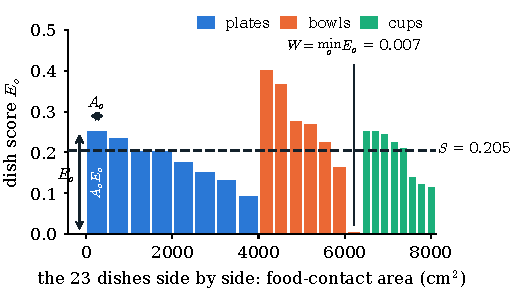
\includegraphics{figures/step5_load.pdf}}
{Step 5 in symbols, on the 23 dishes of the example load (sorted by $E_o$ within each kind). Each dish is a column of width $A_o$ and height $E_o$, so its area is $A_oE_o$. $S=\sum_oA_oE_o/\sum_oA_o$ is the height the colored area would have if spread evenly over the full width (dashed), and $W=\min_oE_o$ is the lowest column (bowl\_03).}

\ifpuddlerule
\head{Puddle rule.}
For dish $o$, let $z_{\mathrm{in}}(o)$ be the height of the lowest point of its food-contact surface and $z_{\mathrm{rim}}(o)$ the height of the lowest point of its rim, both as the dish sits in the rack.
The dish \emph{pools} when
\begin{equation}
z_{\mathrm{in}}(o)<z_{\mathrm{rim}}(o)-\delta_p,
\end{equation}
that is, its inside dips more than a small tolerance $\delta_p$ below the rim's lowest point, so water in the cavity cannot run out over the rim.
$X$ is \emph{feasible} if no dish pools.
This is a pass/fail gate, not a penalty: $S$ is computed the same way, and the goal search (the coordinate ascent that picks the benchmark's target load by moving one dish at a time to another candidate placement) accepts a change only if the result is feasible and raises $S$.
\fi

\head{What $e_j$ approximates.}
With infinitely many spray points, the sums over $k$ in~\eqref{eq:e} become integrals over the disc:
\begin{equation}
e(\vp,\vn)=\frac{\int_{\mathcal{D}_a}\max(0,\vn^\top\vd)\,V\,\mathrm{d}A}{\int_{\mathcal{D}_a}\max(0,\vn^\top\vd)\,\mathrm{d}A}.
\end{equation}
Here $\vp$ and $\vn$ are a dot's position and unit normal (index dropped), $\mathcal{D}_a$ is the disc of its dish's arm, $\mathrm{d}A$ is a small patch of the disc around the integration point $\vq$, $\vd$ is the unit direction from $\vp$ to $\vq$, and $V$ is $1$ if the line from $\vp$ to $\vq$ is open and $0$ if not.
Physical irradiance (power per unit area reaching the dot) from the disc would instead be $\int_{\mathcal{D}_a} L\max(0,\cos\theta_{\vp})\cos\theta_{\vq}\,V\,\lVert\vq-\vp\rVert^{-2}\,\mathrm{d}A$, with $L$ the strength of the source (its radiance), $\theta_{\vp}$ the angle between the line and the dish normal, $\theta_{\vq}$ the angle between the line and the disc's normal (straight up), and $\lVert\vq-\vp\rVert^{-2}$ the inverse-square falloff with distance.
The score differs on purpose in two ways.
(i) It drops $L$, $\cos\theta_{\vq}$ and the falloff, because the directions and strengths of the real jets are unknown, so every disc point counts equally.
(ii) It divides by the unblocked value, so for a dot with at least one front-facing point, $e_j=1$ exactly when none of them is blocked, and $e_j$ measures blocking by dishes and rack wires.
A dot with no front-facing point gets $e_j=0$ by the rule in~\eqref{eq:e}.
Every dish sits above its disc, so a surface whose tangent plane has the whole disc behind it (e.g., the floor of a mouth-up bowl, facing straight up) scores $0$ whatever surrounds it.

\ifproperties
\head{Properties.}
\begin{enumerate}
\item $e_j,E_o,S,W\in[0,1]$ and deterministic: each numerator is at most its denominator, the rest are averages and a minimum, and nothing is random (the line tests run on CPU or GPU, which can disagree on a line that just grazes an edge; this moves $S$ by about $10^{-6}$, so quote $S$ to 3 decimals).
\item Adding a dish never raises another dish's $E$: the denominator of $e_j$ does not change, and more blockers can only turn open lines into blocked ones.
\item $S$ itself is not monotone: adding a dish whose $E$ is below the current $S$ lowers it, adding one whose $E$ is above $S$ and that blocks little of the others raises it, and removing a dish whose $E$ is below $S$ raises it. So compare only complete loads of the same dishes.
\item The two arms separate: if the lower-rack and basket dishes lie below the plane of the middle-arm disc and the upper-rack dishes above it, no line crosses that plane, so each dish's $E$ depends only on dishes of its own arm; as long as no dish changes arm, the area-weighted mean of $E_o$ over one arm's dishes can be raised without changing the other arm's.
\end{enumerate}
\fi

\head{Parameters.}
$N=500$ dots per dish; $K=64$ spray points per disc; $\epsilon=0.1$\,mm;\ifpuddlerule{} $\delta_p=2$\,mm;\fi lower-arm disc: center $(0,\,0.008,\,0.185)$\,m, radius $0.233$\,m; middle-arm disc: center $(0,\,0.008,\,0.540)$\,m, radius $0.191$\,m (disc positions and sizes are assumptions); food-contact areas $A_o=502$, $340$, $215$\,cm$^2$ for a plate, bowl and cup.

{\footnotesize Coordinates: $x$ across the width ($0$ on the center line), $y$ from the door ($-$) to the back ($+$), $z$ up from the kitchen floor (the tub floor is at $z=0.152$\,m).
Source: \texttt{exposure.py} (revision 5, \texttt{frigidaire/src/dishsim\_frigidaire/}); the dots come from \texttt{surface\_samples} there, and the food-contact surface from \texttt{register\_hotec} in \texttt{frigidaire\_hotec\_exposure\_search.py}. An optional ceiling-nozzle source for upper-rack dishes exists in the code with weight 0 (off).\par}

\end{document}
